\documentclass{beamer}
\usepackage{graphicx}
\usepackage[utf8]{inputenc} 
\usepackage[ngerman]{babel}
\usetheme{Warsaw}  %% Themenwahl

% Java Code
\usepackage{listings}
\usepackage{color}

\definecolor{dkgreen}{rgb}{0,0.6,0}
\definecolor{gray}{rgb}{0.5,0.5,0.5}
\definecolor{mauve}{rgb}{0.58,0,0.82}

\lstset{frame=tb,
  language=Java,
  aboveskip=3mm,
  belowskip=3mm,
  showstringspaces=false,
  columns=flexible,
  basicstyle={\small\ttfamily},
  numbers=none,
  numberstyle=\tiny\color{gray},
  keywordstyle=\color{blue},
  commentstyle=\color{dkgreen},
  stringstyle=\color{mauve},
  breaklines=true,
  breakatwhitespace=true
  tabsize=3
}

\title{Spezifikation}
\author{Daniel Riedl}
\date{\today}
 
\begin{document}

	\begin{frame}
		\titlepage
	\end{frame}
	
	\begin{frame}
		\tableofcontents
	\end{frame}
	
\section{Kurze Beschreibung der Klassen und Methoden für die Tests}
	
	\begin{frame}[fragile]
	\frametitle{ComObjects}
	\begin{lstlisting}
	public class ComInitLobby implements ComObject, Serializable {
	private List<String> playerList;
	private Set<GameServerRepresentation> gameList;
    public ComInitLobby(List<String> playerList, Set gameList) {
        this.playerList = playerList;
        this.gameList = gameList;
    }
	...
    public void process(ClientModel model) {
        model.receiveMessage(this);
    }
    public void process(Player player, Server server) {
        server.receiveMessage(player,this);
    }
	\end{lstlisting}
	\end{frame}
	
	\begin{frame}[fragile]
	\frametitle{Receive/Send Messages}
	\begin{lstlisting}
	public class ClientModell extends Observable{
		...
		public void receiveMessage(ComRuleset msg) {
		public void receiveMessage(ComInitGameLobby msg) {}
		public void send(RulesetMessage msg) {}
		public void send(ComObject object) {}
		...}
	public class MessageListenerThread extends Thread {
		...
		public void run() {
			...
			object = (ComObject) in.readObject();
			object.process(model);
			...}
	}		
	\end{lstlisting}
	\end{frame}
	
	\begin{frame}[fragile]
	\frametitle{Ruleset}
	\begin{lstlisting}
		public abstract class ServerRuleset {
			private GameServer server;
			private GameState gameState;
			private GamePhase gamePhase;
			...
			public void runGame() {}
			public void resolveMessage(MsgCard msgCard, String name) {}
			protected abstract boolean isValidMove(Card card);
			protected abstract void calculateTricks();
			protected abstract void calculateRoundOutcome();		
	\end{lstlisting}
	\end{frame}
	
\section{DummyKlassen}
	
	\begin{frame}[fragile]
		\frametitle{DummyKlassen}
		\begin{itemize}
			\item TestGameServer
			\item TestLobbyServer
			\item TestMessageListenerThread
			\item TestObserver
			\item TestPlayer
		\end{itemize}

	\end{frame}
	\begin{frame}[fragile]
		\frametitle{TestPlayer}
\begin{lstlisting}
public class TestPlayer extends Player {
	...
	private List<ComObject> inputComObject;	
	public List<ComObject> getServerInput() {
		return inputComObject;
	}	
	public void injectComObject(ComObject object) {
		object.process(this, server);
	}
	public void send(ComObject com) {
		inputComObject.add(com);
	}
	...
}
}

\end{lstlisting}
	\end{frame}
\section{Tests}

\begin{frame}
\frametitle{Wizard}
	\begin{block}
		{Wizard} Bei einem Spiel Wizard wo die erste Karte bereits auf dem Tisch liegt, soll geprüft werden dass nur noch regelkonforme Karten gespielt werden können
	\end{block}
\end{frame}

	\begin{frame}[fragile]
	\frametitle{Wizard}
	\begin{lstlisting}
public class TestisValidMoveWizard {
	@Before
	public void setUp() throws Exception {
		player1 = "Tick";
		...
		lobbyServer = new TestLobbyServer();
		player = new TestPlayer(lobbyServer,null,null);
		gameServer = new TestGameServer(lobbyServer,player,"Mein Spiel",RulesetType.Wizard, "", false);
		ruleset = new ServerWizard(gameServer);				
		ruleset.addPlayerToGame(player1);
		ruleset.addPlayerToGame(player2);
        ...		
	\end{lstlisting}	
	
	\end{frame}
	
	\begin{frame}[fragile]
	\frametitle{Wizard}
	\begin{lstlisting}
		playerState1 = ruleset.getPlayerState(player1);
		...	
		ruleset.setFirstPlayer(playerState1);
		ruleset.setTrumpCard(WizardCard.VierRot);
		
		ruleset.giveACard(playerState1, WizardCard.DreiGruen);
		ruleset.giveACard(playerState1, WizardCard.ZaubererRot);
		
		ruleset.giveACard(playerState2, WizardCard.ZweiGruen);
		ruleset.giveACard(playerState2, WizardCard.DreiRot);
		...
	\end{lstlisting}
	
	\end{frame}	
	
	\begin{frame}[fragile]
	\frametitle{Wizard}
	\begin{lstlisting}
	@Test
	public void testRed3OnGreen3() {
		ruleset.playCard(WizardCard.DreiGruen);
		ruleset.setCurrentPlayer(playerState2);	
		assertFalse(ruleset.isValidMove(WizardCard.DreiRot));
	}
	@Test
	public void testGreen2OnGreen3() {
		ruleset.playCard(WizardCard.DreiGruen);
		ruleset.setCurrentPlayer(playerState2);				
		assertTrue(ruleset.isValidMove(WizardCard.ZweiGruen);
	}
	\end{lstlisting}
	
	\end{frame}

\begin{frame}
\frametitle{Hearts}
	\begin{block}
		{Hearts} Es wurde noch keine Karte in Hearts gespielt. Der Spieler der zuerst spielt, darf nur ein Herz spielen wenn er keine andere Farbe mehr hat.
	\end{block}
\end{frame}

\begin{frame}[fragile]
\frametitle{Hearts}
\begin{lstlisting}
	@Test
	public void testIsValidMove() {
		 ruleset.giveACard(playerState1, HeartsCard.Herz2);
	     ruleset.giveACard(playerState1, HeartsCard.Kreuz9)
	     ...    
	     assertFalse(ruleset.isValidMove(HeartsCard.Herz2));     
	     assertTrue(ruleset.isValidMove(HeartsCard.Caro3););
	}
\end{lstlisting}
\end{frame}



\begin{frame}[fragile]
\frametitle{Hearts}
\begin{lstlisting}
	@Test
	public void testIsValidMoveOnlyHearts() {
		 ruleset.giveACard(playerState1, HeartsCard.Herz2);
	     ruleset.giveACard(playerState1, HeartsCard.Herz5);
	     ...     
	     assertTrue(ruleset.isValidMove(HeartsCard.Herz2));     
	     assertTrue(ruleset.isValidMove(HeartsCard.Herz5));
	}
\end{lstlisting}
\end{frame}


\begin{frame}
\frametitle{Siegerbestimmung}
	\begin{block}
		{Siegerbestimmung} Bei einem Spiel muss bei Spielende der korrekte Sieger bestimmt werden und an alle Mitspieler weitergeleitet werden.
	\end{block}
\end{frame}


\begin{frame}[fragile]
\frametitle{Siegerbestimmung bei Hearts}
\begin{lstlisting}
	@Before
	public void setUp() {
		lobbyServer = new LobbyServer();
		blue = new TestPlayer(lobbyServer, null, null);
		white = new TestPlayer(lobbyServer, null, null);
		...
	}
	@Test
	public void testGetWinner() {		
		gameServer = new GameServer(lobbyServer, blue, "Test Game", 		  RulesetType.Hearts, "", false);
		gameServer.addPlayer(white);
		...		
		heartsServerRuleset = new ServerHearts(gameServer);
		...
\end{lstlisting}
\end{frame}


\begin{frame}[fragile]
\frametitle{Siegerbestimmung bei Hearts}
\begin{lstlisting}
	heartsServerRuleset.addPlayerToGame("Mr. Blue");
	...
		heartsServerRuleset.setPoints(heartsServerRuleset.getPlayerState("Mr. White"),20);
		...
		heartsServerRuleset.setPoints(heartsServerRuleset.getPlayerState("Mr. Brown"),110);
		
		heartsServerRuleset.setGamePhase(GamePhase.Ending);
		heartsServerRuleset.calculateRoundOutcome();		
		assertTrue(heartsServerRuleset.getWinner().equals("Mr. White"));		
		...
\end{lstlisting}
\end{frame}



\begin{frame}[fragile]
\frametitle{Siegerbestimmung bei Hearts}
\begin{lstlisting}
		inputList = blue.getServerInput();
		comObject = (ComRuleset) inputList.get(1);
		endMsg = (MsgGameEnd) comObject.getRulesetMessage();
		winner = endMsg.getWinner();
		assertEquals("Nachricht an Blue", "Mr. White", winner);

		inputList = white.getServerInput();
		comObject = (ComRuleset) inputList.get(1);
		endMsg = (MsgGameEnd) comObject.getRulesetMessage();
		winner = endMsg.getWinner();
		assertEquals("Nachricht an White", "Mr. White", winner);
		...
\end{lstlisting}
\end{frame}

\begin{frame}[fragile]
\frametitle{Siegerbestimmung bei Hearts}
\begin{lstlisting}
		inputList = blue.getServerInput();
		comObject = (ComRuleset) inputList.get(1);
		endMsg = (MsgGameEnd) comObject.getRulesetMessage();
		winner = endMsg.getWinner();
		assertEquals("Nachricht an Blue", "Mr. White", winner);

		inputList = white.getServerInput();
		comObject = (ComRuleset) inputList.get(1);
		endMsg = (MsgGameEnd) comObject.getRulesetMessage();
		winner = endMsg.getWinner();
		assertEquals("Nachricht an White", "Mr. White", winner);
		...
\end{lstlisting}
\end{frame}

\begin{frame}
\frametitle{Spieler verlässt Spiel}
	\begin{block}
		{Spieler verlässt Spiel} Wenn ein Spieler ein Spiel verlässt, müssen alle anderen Spieler benachrichtigt werden und zurück in die Lobby gebracht werden.
	\end{block}
\end{frame}

\begin{frame}[fragile]
\frametitle{Spieler verlässt Spiel}
\begin{lstlisting}
		@Before
		public void setUp() throws Exception {
		lobby = new TestLobbyServer();
		player1 = new TestPlayer(lobby, null, null);
		player1.setName("MrBlue");
		lobby.addPlayer(player1);		
		player2 = new TestPlayer(lobby, null, null);
		player2.setName("MrWhite");
	   ...	
		game = new TestGameServer(lobby, player1, "MrBluesGame", RulesetType.Hearts, null, false);	
		game.addPlayer(player2);
		game.addPlayer(player3);
		game.addPlayer(player4);
		
		quit = new ComClientQuit();
	}
\end{lstlisting}
\end{frame}


\begin{frame}[fragile]
\frametitle{Spieler verlässt Spiel}
\begin{lstlisting}
	@Test
	public void testPlayerQuitGame() throws IOException{ 	
		player1.changeServer(game);
		assertTrue(game.initLobby().getPlayerList().
		    contains(player1.getName()));
		
		player1.injectComObject(quit);

		assertFalse(lobby.initLobby().getGameList().contains(game));
		assertTrue(lobby.initLobby().getPlayerList().
		    contains(player1.getName()));
		assertTrue(lobby.initLobby().getPlayerList().
		    contains(player2.getName()));
		...
\end{lstlisting}
\end{frame}

\begin{frame}
\frametitle{Chat}
	\begin{block}
		{Chat} Nachrichten die vom Client an den Server geschickt werden, müssen an
		allen anderen Clients die sich im Server befinden ankommen.
	\end{block}
\end{frame}

\begin{frame}[fragile]
\frametitle{ChatModel}
\begin{lstlisting}
	@Before  
    public void setUp() {
		testNetIO = new TestMessageListenerThread();
		testObserver = new TestObserver();
		testMessage = new ComChatMessage("Hello Test!");
		testModel = new ClientModel((MessageListenerThread) testNetIO);
		testNetIO.setModel(testModel);
		testModel.addObserver(testObserver);
    }
\end{lstlisting}
\end{frame}


\begin{frame}[fragile]
\frametitle{ChatModel}
\begin{lstlisting}
	@Test
	public void testSendChatMessage() {
		String inputText = "Hello Test!";
		testModel.sendChatMessage(inputText);
		testText = ((ComChatMessage) 			testNetIO.getModelInput().get(0)).getChatMessage();
		assertEquals("Vergleich der gesendeten Chatnachrichten", testText, inputText);
	}	
	@Test
	public void testReceiveChatMessage() {
		testNetIO.injectComObject(testMessage);
		assertTrue("Vergleich der empfangenen Chatnachrichten", 
				testObserver.getChatMessage().
				equals(testMessage.getChatMessage()));
	}
\end{lstlisting}
\end{frame}


\begin{frame}[fragile]
\frametitle{ChatServer}
\begin{lstlisting}
	@Before
	public void setUp() {
		testMessage = new ComChatMessage("Hello Test!");
		testServer = new LobbyServer();
		player1 = new TestPlayer(testServer, null, null);
		player2 = new TestPlayer(testServer, null, null);
	}
\end{lstlisting}
\end{frame}


\begin{frame}[fragile]
\frametitle{ChatServer}
\begin{lstlisting}
	@Test
	public void testReceiveMessagePlayerComChatMessage() {
		String messageToMatch = testMessage.getChatMessage();
		testServer.addPlayer(player1);
		testServer.addPlayer(player2);
		player1.injectComObject(testMessage);
		testText1 = ((ComChatMessage) player1.getServerInput(0)).getChatMessage();
		testText2 = ((ComChatMessage) player2.getServerInput(0)).getChatMessage();
		assertEquals("Nachricht an Spieler 1", messageToMatch, testText1);
		assertEquals("Nachricht an Spieler 2", messageToMatch, testText2);
	}
\end{lstlisting}
\end{frame}

\section{Implmentierungsplan}

\begin{frame}
\frametitle{Milestone 1 (27.11.2013)}
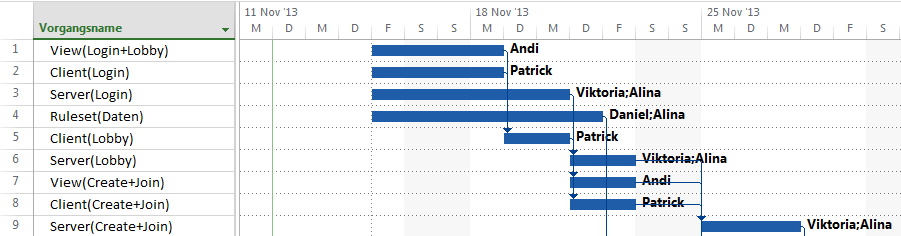
\includegraphics[scale=0.48]{Milestone1}
\end{frame}

\begin{frame}
\frametitle{Milestone 2 (04.12.2013)}
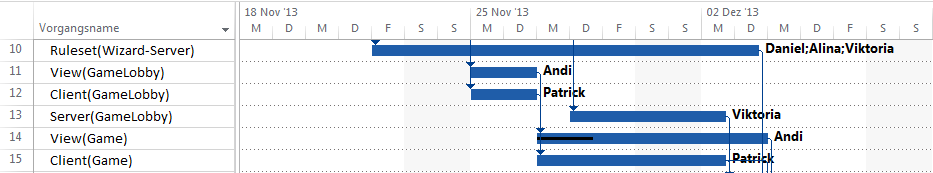
\includegraphics[scale=0.48]{Milestone2}
\end{frame}

\begin{frame}
\frametitle{Milestone 3 (11.12.2013)}
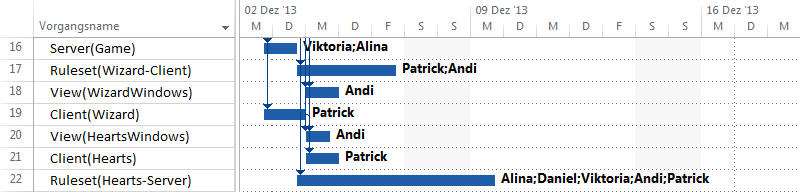
\includegraphics[scale=0.48]{Milestone3}
\end{frame}

\begin{frame}
\frametitle{Finale Version (17.12.2013)}
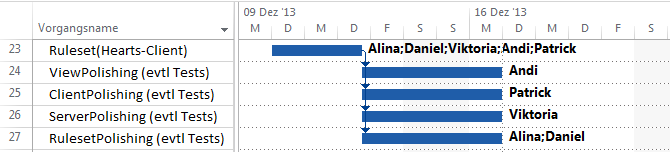
\includegraphics[scale=0.48]{Milestone4}
\end{frame}

	
\end{document}